\documentclass[compress,red]{beamer}
\usepackage[utf8]{inputenc}
\usepackage{ucs}
\usepackage{amsmath}
\usepackage{amsfonts}
\usepackage{amssymb}
\usepackage[russian]{babel}
\usepackage{graphicx}
\usepackage{wrapfig}

\usepackage{tikz}
\usepackage{verbatim}

\usepackage{color}
\usepackage{xcolor}
\usepackage{listings}

\usepackage{caption}

\lstset{
language=sql,
extendedchars=\true,
inputencoding=utf8x,
commentstyle=\itshape,
stringstyle=\bf,
belowcaptionskip=5pt }


\DeclareCaptionFont{white}{\color{white}}
\DeclareCaptionFormat{listing}{\colorbox{gray}{\parbox{\textwidth}{#1#2#3}}}
\captionsetup[lstlisting]{format=listing,labelfont=white,textfont=white}

\usetikzlibrary{calc,trees,positioning,arrows,chains,shapes.geometric,%
    decorations.pathreplacing,decorations.pathmorphing,shapes,%
    matrix,shapes.symbols}

\tikzset{
>=stealth',
  punktchain/.style={
    rectangle, 
    rounded corners, 
    % fill=black!10,
    draw=black, very thick,
    text width=10em, 
    minimum height=3em, 
    text centered, 
    on chain},
  line/.style={draw, thick, <-},
  element/.style={
    tape,
    top color=white,
    bottom color=blue!50!black!60!,
    minimum width=8em,
    draw=blue!40!black!90, very thick,
    text width=10em, 
    minimum height=1.5em, 
    text centered, 
    on chain},
  every join/.style={->, thick,shorten <=1pt},
  decoration={brace},
  tuborg/.style={decorate},
  tubnode/.style={midway, right=2pt},
}

\mode<presentation>

\usetheme{Warsaw}

\definecolor{Red}{rgb}{1,0,0}
\definecolor{Blue}{rgb}{0,0,1}
\definecolor{Green}{rgb}{0,1,0}
\definecolor{magenta}{rgb}{1,0,.6}
\definecolor{lightblue}{rgb}{0,.5,1}
\definecolor{lightpurple}{rgb}{.6,.4,1}
\definecolor{gold}{rgb}{.6,.5,0}
\definecolor{orange}{rgb}{1,0.4,0}
\definecolor{hotpink}{rgb}{1,0,0.5}
\definecolor{newcolor2}{rgb}{.5,.3,.5}
\definecolor{newcolor}{rgb}{0,.3,1}
\definecolor{newcolor3}{rgb}{1,0,.35}
\definecolor{darkgreen1}{rgb}{0, .35, 0}
\definecolor{darkgreen}{rgb}{0, .6, 0}
\definecolor{darkred}{rgb}{.75,0,0}

\xdefinecolor{olive}{cmyk}{0.64,0,0.95,0.4}
\xdefinecolor{purpleish}{cmyk}{0.75,0.75,0,0}

\useoutertheme[subsection=false]{smoothbars}

\title{Реляционные базы данных}
\author{Информатика \\ 10-11 классы}

%\usecolortheme{dolphin}


\begin{document}
%%титульная страница
\maketitle
%% основные моменты

\section{Введение}

\subsection{Базы данных}
\begin{frame}[fragile]
  \frametitle{Базы данных}
  \begin{itemize}
    \item С ростом количества информации возникают сложности с её хранением и обработкой.
    \item Имея, к примеру, на компьютере один пароль, его легко запомнить. Имея же их 100500, памяти уже может не хватить.
    \item Многие вещи сейчас мы уже и не стараемся запомнить.
    \item Например, кто из вас помнит наизусть мобильный телефон родителей? А друзей? А родственников?
    \item Для хранения и удобного доступа к информации давно используются \textbf{базы данных}.
  \end{itemize}
\end{frame}

\subsection{Примеры}
\begin{frame}[fragile]
  \frametitle{Какие базы данных существуют?}
  \begin{itemize}[<+->]
    \item телефонная книга,
    \item журнал,
    \item список e-mail'ов,
    \item база данных жителей России (привет, ВКонтакте),
    \item тысячи их...
  \end{itemize}
\end{frame}

\subsection{Типы баз данных}
\begin{frame}
  \begin{center}
    \Huge{Типы баз данных и систем базы данных}
  \end{center}
  \begin{center}
    \begin{itemize}
      \item \Large{Реляционная (табличная)}
      \item \Large{Иерархическая}
      \item \Large{Объектная}
      \item \Large{Сетевая}
    \end{itemize}
  \end{center}
\end{frame}

\section{Табличные базы данных}
\subsection{Табличные БД}
\begin{frame}
  \begin{center}
    \Huge{Табличные базы данных}
  \end{center}
\end{frame}

\subsection{Пример табличной БД}
\begin{frame}[fragile]
  \frametitle{Пример табличной базы данных}
  \begin{center}
    \begin{tabular}{|c|c|c|c|}
    \hline
    \textbf{Имя} & \textbf{Фамилия} & \textbf{Телефон} & \textbf{Город}\\
    \hline
    Вася & Васильев & 1234567 & Санкт-Петербург\\
    \hline
    Петя & Петров & 2345678 & Санкт-Петербург\\
    \hline
    Фёдор & Фёдоров & 3456789 & Москва\\
    \hline
    \end{tabular}
  \end{center}
\end{frame}

\subsection{Разбор табличной БД}
\begin{frame}[fragile]
  \frametitle{Составные части}
  \centerline{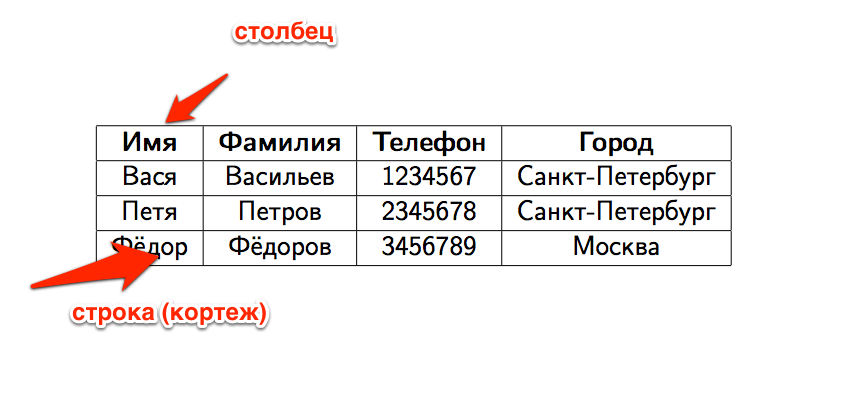
\includegraphics[width=0.8\textwidth]{images/database_part1.png}}
  \begin{itemize}
    \item столбцы,
    \item строки (\emph{кортежи}, записи)
  \end{itemize}
\end{frame}

\subsection{Реальная БД}
\begin{frame}[fragile]
  \frametitle{Пример реальной базы}
  \centerline{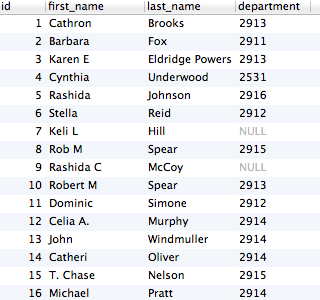
\includegraphics[width=0.5\textwidth]{images/database_part2.png}}
\end{frame}

\subsection{СУБД}
\begin{frame}[fragile]
  \frametitle{СУБД}
  \begin{itemize}
    \item СУБД (система управления базами данных) --- совокупность программ, обеспечивающих управление базами данных.
    \item Есть множество СУБД: \textbf{MySQL}, PostgreSQL, Oracle, MS SQL Server, IBM DB2, Interbase, Microsoft Access и др.
    \item Здесь и далее мы будем в качестве основной рассматривать СУБД MySQL. 
    \item Тем не менее, мы будем использовать для работы с БД язык SQL 92, поэтому большая часть запросов будет применима и для других SQL-ориентированных баз данных (например, PostgreSQL или MS SQL Server).
    \item MySQL: http://mysql.com (свободная СУБД)
  \end{itemize}
\end{frame}

\subsection{Типы данных}
\begin{frame}[fragile]
  \frametitle{Основные типы данных}
  В MySQL существуют достаточно типов данных, мы же перечислим основные:
  \begin{tabular}{|l|l|}
  \hline
  Название & Пояснение\\
  \hline
  TINYINT & Целое число от -128 до 127\\
  \hline
  INT & Целое число от -2147483648 до 2147483648\\
  \hline
  FLOAT & вещественное число\\
  \hline
  DOUBLE & вещественное число повышенной точности\\
  \hline
  DATE & дата\\
  \hline
  DATETIME & дата и время\\
  \hline
  TIMESTAMP & кол-во секунд, прошедшее с 1970-01-01 00:00:00\\
  \hline
  VARCHAR & строка заданной длины (до 255 символов)\\
  \hline
  TEXT & текст\\
  \hline
  \end{tabular}
\end{frame}

\section{SQL}
\subsection{SQL}
\begin{frame}
  \begin{center}
    \Huge{SQL}
  \end{center}
  \begin{center}
    \Large{Structured Query Language}
  \end{center}
\end{frame}

\subsection{Описание SQL}
\begin{frame}[fragile]
  \frametitle{Что такое SQL?}
  \begin{itemize}
    \item SQL --- универсальный язык запросов к реляционным базам данных.
    \item SQL был разработан для выполнения следующих операций:
      \begin{enumerate}
        \item создание новой таблицы,
        \item создание новой записи в таблице,
        \item изменение записей,
        \item удаление записей,
        \item выборка записей из одной или нескольких таблиц,
        \item изменение структуры таблицы.
      \end{enumerate}
  \end{itemize}
\end{frame}

\subsection{Первичный ключ}
\begin{frame}[fragile]
  \frametitle{Первичный ключ}
  \begin{itemize}
    \item Прежде чем перейти непосредственно к языку, укажем несколько полезных правил (по-хорошему, это называется \emph{нормальными формами}).
    \item Записи в таблице должны отличаться друг от друга. Уникальное поле или набор полей, отличающее одну запись от другой, называется \emph{первичным ключом}.
    \item Вводя первичный ключ, мы должны быть уверены в его надёжности. Например, имя и фамилия — плохие первичные ключи, так как умеют повторяться.
    \item А вот номер паспорта --- отличный первичный ключ.
    \item Часто поступают ещё проще: вводят специальный столбец \textbf{id}, который содержит номер записи, который последовательно увеличивается.
  \end{itemize}
\end{frame}

\subsection{Тестовая таблица}
\begin{frame}[fragile]
  \frametitle{Тестовая таблица users}
  \begin{tabular}{|c|c|c|c|c|}
  \hline
  id & first\_name & last\_name & gender & created\_at\\
  \hline
  1 & Ivan & Ivanov & 1 & 2012-01-01\\
  \hline
  2 & Sasha & Petrov & 1 & 2012-01-02\\
  \hline
  3 & Masha & Mashakova & 2 & 2012-01-01\\
  \hline
  4 & Sasha & Simonov & 1 & 2012-05-1\\
  \hline
  5 & Sidor & Sidorov & 1 & 2012-07-01\\
  \hline
  6 & Sasha & Pimenova & 2 & 2012-04-02\\
  \hline
  \end{tabular}
\end{frame}

\section{SELECT}
\subsection{Оператор SELECT}
\begin{frame}[fragile]
  \frametitle{Оператор SELECT}
  \begin{itemize}
    \item Оператор SELECT позволяет сделать выборку записей из базы данных.
    \item Синтаксис:
    \scriptsize{
    \begin{lstlisting}[label=sql1,caption=Синтаксис SELECT]
      SELECT %fields% FROM %table%
                      WHERE %conditions%
                      ORDER BY %fields% ASC/DESC
                      LIMIT %limit%, %offset%
    \end{lstlisting}
    }
    \item limit --- сколько брать записей, offset --- начиная с какой?
  \end{itemize}
\end{frame}

\subsection{Пример запроса}
\begin{frame}[fragile]
  \frametitle{Пример запроса}
  \begin{tabular}{|c|c|c|c|c|}
  \hline
  id & first\_name & last\_name & gender & created\_at\\
  \hline
  \end{tabular}
  \begin{itemize}
    \item Выведем на экран имена и фамилии всех мужчин:
  \end{itemize}
  \scriptsize{
  \begin{lstlisting}[label=sql2,caption=SELECT]
    SELECT first_name, last_name FROM users
    WHERE (gender = 1)
  \end{lstlisting}
  }
\end{frame}

\subsection{Пример запроса 2}
\begin{frame}[fragile]
  \frametitle{Пример запроса с двумя условиями}
  \begin{tabular}{|c|c|c|c|c|}
  \hline
  id & first\_name & last\_name & gender & created\_at\\
  \hline
  \end{tabular}
  \begin{itemize}
    \item Выведем на экран список всех Саш--мужчин:
  \end{itemize}
  \scriptsize{
  \begin{lstlisting}[label=sql3,caption=SELECT]
    SELECT * FROM users
    WHERE (gender = 1) AND (first_name = "Sasha")
  \end{lstlisting}
  }
\end{frame}

\subsection{Пример запроса 3}
\begin{frame}[fragile]
  \frametitle{Первая зарегистрированная женщина}
  \begin{tabular}{|c|c|c|c|c|}
  \hline
  id & first\_name & last\_name & gender & created\_at\\
  \hline
  \end{tabular}
  \begin{itemize}
    \item А если мы хотим вывести первую зарегистрированную женщину?
  \end{itemize}
  \scriptsize{
  \begin{lstlisting}[label=sql4,caption=SELECT]
    SELECT * FROM users
    WHERE (gender = 2)
    ORDER BY created_at
    LIMIT 1
  \end{lstlisting}
  }
\end{frame}

\subsection{Пример запроса 3}
\begin{frame}[fragile]
  \frametitle{Первая зарегистрированная женщина}
  \begin{tabular}{|c|c|c|c|c|}
  \hline
  id & first\_name & last\_name & gender & created\_at\\
  \hline
  \end{tabular}
  \begin{itemize}
    \item А последнего мужчину?
  \end{itemize}
  \scriptsize{
  \begin{lstlisting}[label=sql5,caption=SELECT]
    SELECT * FROM users
    WHERE (gender = 1)
    ORDER BY created_at DESC
    LIMIT 1
  \end{lstlisting}
  }
\end{frame}

\subsection{Пример запроса 3}
\begin{frame}[fragile]
  \frametitle{Первая зарегистрированная женщина}
  \begin{tabular}{|c|c|c|c|c|}
  \hline
  id & first\_name & last\_name & gender & created\_at\\
  \hline
  \end{tabular}
  \begin{itemize}
    \item А предпоследнего?
  \end{itemize}
  \scriptsize{
  \begin{lstlisting}[label=sql6,caption=SELECT]
    SELECT * FROM users
    WHERE (gender = 2)
    ORDER BY created_at DESC
    LIMIT 1, 1
  \end{lstlisting}
  }
\end{frame}

\subsection{Вторая тестовая таблица}
\begin{frame}[fragile]
  \frametitle{Тестовая таблица courses}
  \begin{tabular}{|c|c|c|c|c|c|c|}
  \hline
  id & title & desc & type & is\_active & created\_at & updated\_at\\
  \hline
  1 & Ruby & ... & 1 & 1 & 2012-01-01 & 2012-01-01\\
  \hline
  2 & Info & ... & 0 & 0 & 2012-01-02 & 2012-02-01\\
  \hline
  3 & Google & ... & 1 & 0 & 2012-03-25 & 2012-05-28\\
  \hline
  4 & Test & ... & 0 & 1 & 2012-03-25 & 2012-11-13\\
  \hline
  \end{tabular}
\end{frame}

\end{document}